\documentclass{article}
\usepackage{amsmath,amssymb,amsthm,mdframed,kotex}
\newcommand{\C}{\ensuremath{\angle C}}
\newcommand{\bb}{\ensuremath{\angle B}}
\newcommand{\D}{\ensuremath{{}^\circ}}
\newcommand{\PP}{\ensuremath{a^2+b^2=c^2}}
\newcommand{\PPP}{\ensuremath{a^2+b^2>c^2}}
\newcommand{\PPPP}{\ensuremath{a^2+b^2<c^2}}
\renewcommand*{\proofname}{증명}
\renewcommand{\figurename}{그림}
\begin{document}
\title{삼각형의 각과 변 사이의 관계}
\date{\today}
\author{}
\maketitle
\tableofcontents

\newpage
%새 節
\section{가정}
평면 위의 세 점 \(A\), \(B\), \(C\)는 삼각형을 이룬다.
각 꼭지점에 대한 대변對邊을 각각 \(a\), \(b\), \(c\)라고 하자.
[그림 1]
\begin{figure}[h]
\center
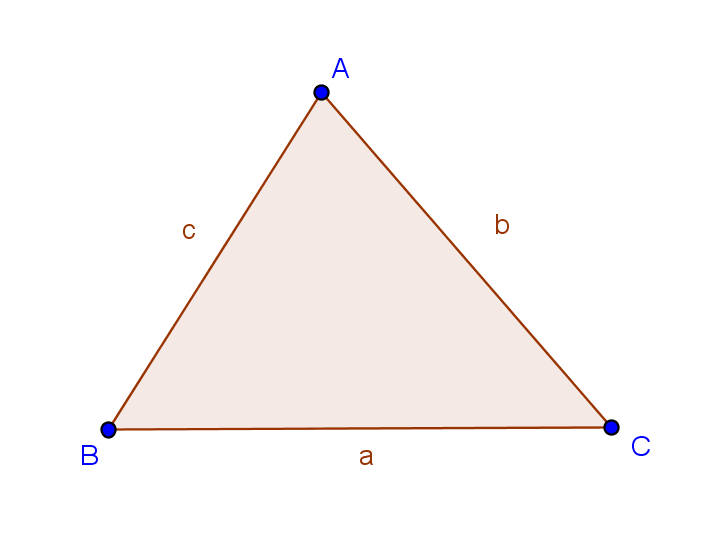
\includegraphics{1}
\caption{삼각형 \(ABC\)}
\end{figure}

%새 節
\section{삼각부등식}
삼각형을 이루는 세 변 \(a\), \(b\), \(c\)에 대해서 다음 부등식이 성립한다.
\begin{gather*}
a+b>c\\
b+c>a\\
c+a>b
\end{gather*}
특히, 한 문자에 관해서 부등식을 풀어내면
\begin{gather*}
c-b<a<c+b\\
c-a<b<c+a\\
b-a<c<b+a
\end{gather*}
이 된다.

\begin{proof}
아래 그림과 같이[그림 2] 반직선 \(\overrightarrow{BA}\) 위에 \(\overline{AD}=\overline{AC}\)가 되는 점 \(D\)를 잡으면 \(\angle DCA<\angle DCB\)가 성립한다.
\(\overline{AD}=\overline{AC}\)이므로 \(\angle DCA=\angle BDC\)이고, 따라서 \(\angle BDC<\angle DCB\)가 성립한다.
삼각형 \(DBC\)에서, 대각의 크기가 크면 대변의 길이도 크므로 \(\overline{BC}<\overline{BD}\)이다.
따라서
\(
c+b
=
\overline{AB}+\overline{AC}
=\overline{AB}+\overline{AD}
=\overline{BD}
>\overline{BC}
=a
\)
가 성립한다.
나머지 두 식도 똑같은 방식으로 증명할 수 있다.
\begin{figure}[h]
\center
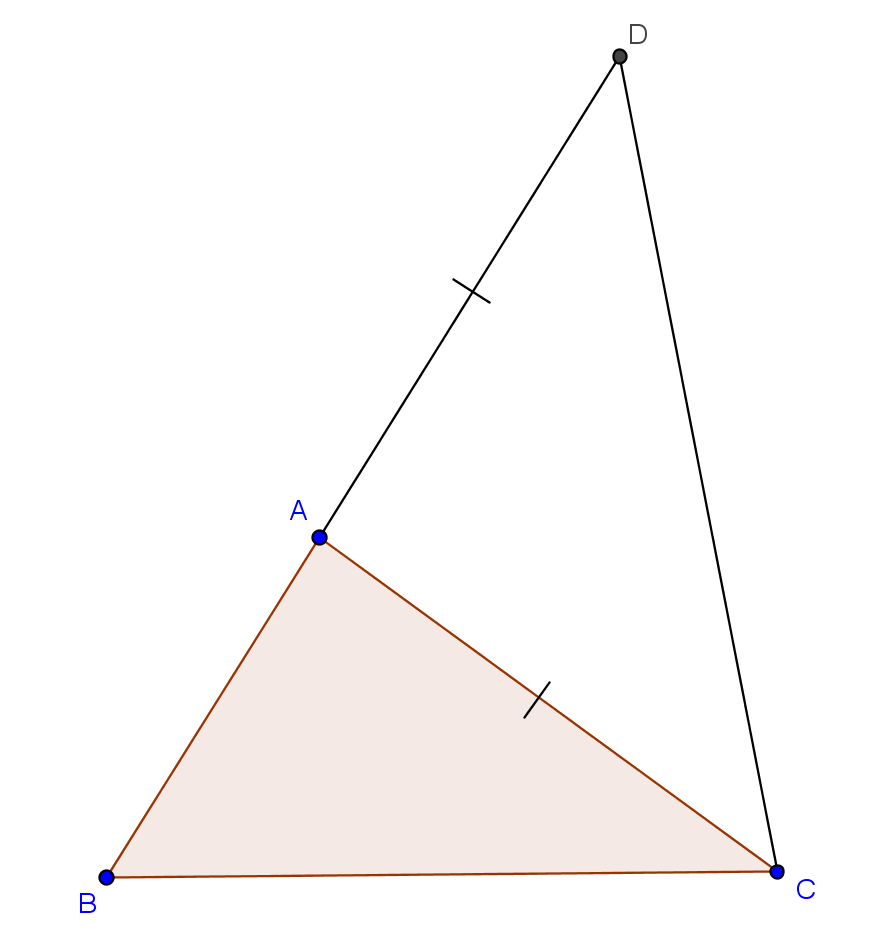
\includegraphics{2}
\caption{삼각부등식의 증명}
\end{figure}
\end{proof}

%새 節
\section{피타고라스의 정리 외}

%새 小節
\subsection{\C=90\D이면 \PP이다(피타고라스의 정리).}
증명은 생략한다.
대표적으로 유클리드의 증명방법이 있다.

%새 小節
\subsection{\C<90\D이면 \PPP이다.}
\begin{proof}
\bb의 크기에 따라 \bb<90\D일 때, \bb=90\D, \bb>90\D일 때로 나누어 생각한다.

i) \bb<90\D일 때

그림 3과 같이 \(A\)에서 \(\overline{BC}\)에 내린 수선의 발을 \(H\), 수선의 길이를 \(h\), \(\overline{CH}\)의 길이를 \(l\)이라고 하면
\begin{figure}[h]
\center
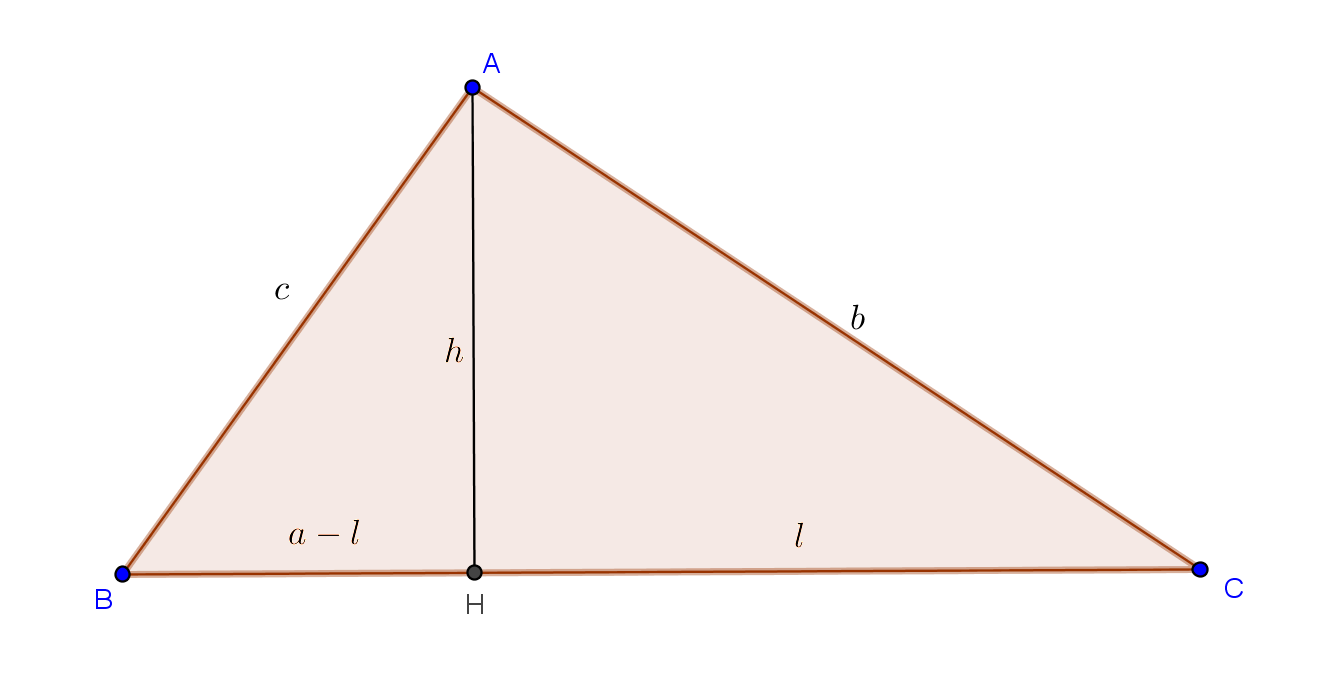
\includegraphics{3_1}
\caption{\C=90\D이고 \bb<90\D일 때}
\end{figure}
\begin{align*}
c^2
&=(a-l)^2+h^2=a^2-2al+l^2+h^2\\
&<a^2+l^2+h^2=a^2+b^2
\end{align*}
이 된다.

ii) \bb=90\D일 때

그림 4에서
\(c^2=b^2-a^2<b^2+a^2\)이다.
\begin{figure}[h]
\center
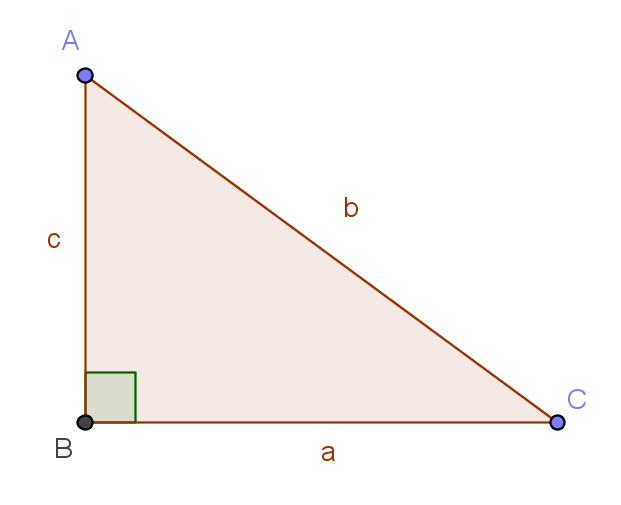
\includegraphics{3_2}
\caption{\C=90\D이고 \bb=90\D일 때}
\end{figure}

iii) \bb>90\D일 때

i)에서와 마찬가지로 \(A\)에서 \(\overline{BC}\)에 내린 수선의 발을 \(H\), 수선의 길이를 \(h\), \(\overline{CH}\)의 길이를 \(l\)이라고 하면
\begin{align*}
c^2
&=(l-a)^2+h^2=a^2-2al+l^2+h^2\\
&<a^2+l^2+h^2=a^2+b^2
\end{align*}
이 된다.[그림 5]
\begin{figure}[h!]
\center
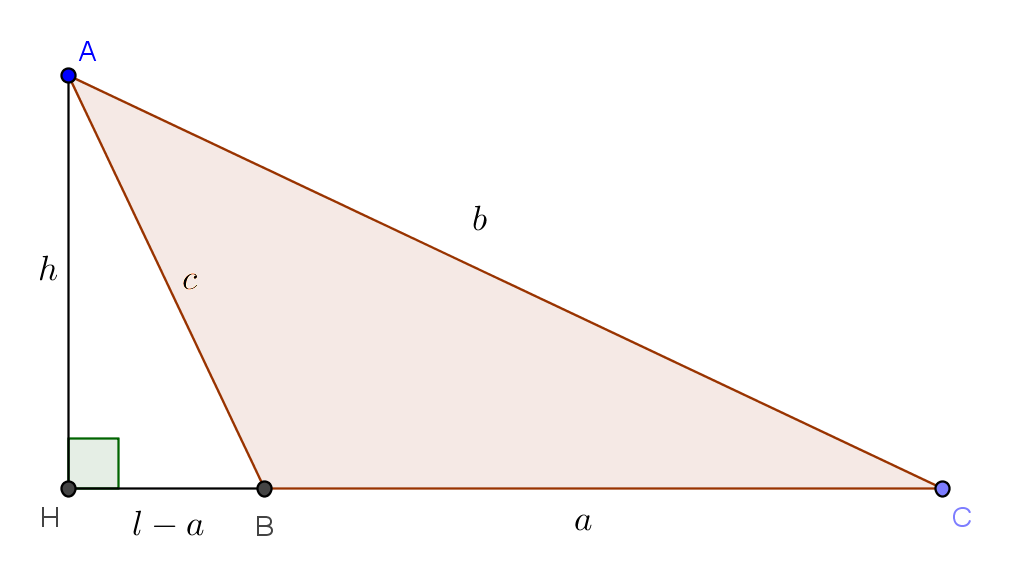
\includegraphics{3_3}
\caption{\C=90\D이고 \bb>90\D일 때}
\end{figure}
\end{proof}

%새 小節
\subsection{\C>90\D이면 \PPPP이다.}
\begin{proof}
\textbf{3.2}절의 i)과 iii)에서와 마찬가지로 \(A\)에서 \(\overline{BC}\)에 내린 수선의 발을 \(H\), 수선의 길이를 \(h\), \(\overline{CH}\)의 길이를 \(l\)이라고 하면
\begin{figure}[h]
\center
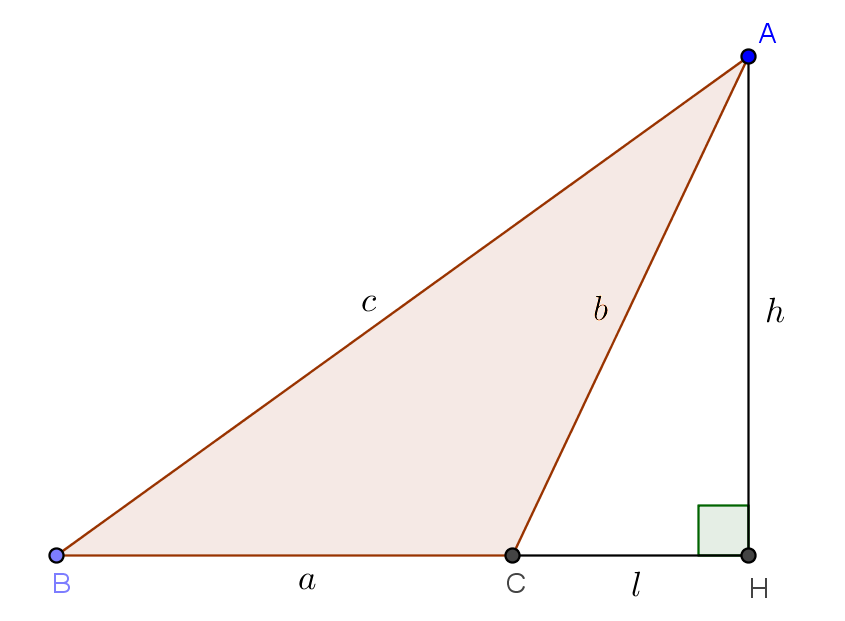
\includegraphics{3_4}
\caption{\C>90\D일 때}
\end{figure}
\begin{align*}
c^2
&=(a+l)^2+h^2=a^2+2al+l^2+h^2\\
&>a^2+l^2+h^2=a^2+b^2
\end{align*}
이 된다.
[그림 6]
\end{proof}

%새 小節
\subsection{\PP이면 \C=90\D이다(피타고라스의 정리의 역).}
\begin{proof}(1)
그림 7과 같이 삼각형 \(ABC\)가 주어져 있고 \PP가 성립한다.
이 삼각형에서 \C=90\D라는 것을 증명해야 한다.
\begin{figure}[h]
\center
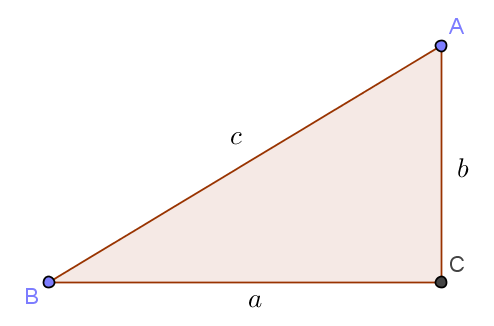
\includegraphics{3_5_1}
\caption{피타고라스 정리의 역에 대한 증명(1)}
\end{figure}

직각을 낀 두 변의 길이가 각각 \(a\), \(b\)인 직각삼각형 \(A'B'C'\)를 아래 그림 8과 같이 그린다.
\begin{figure}[h]
\center
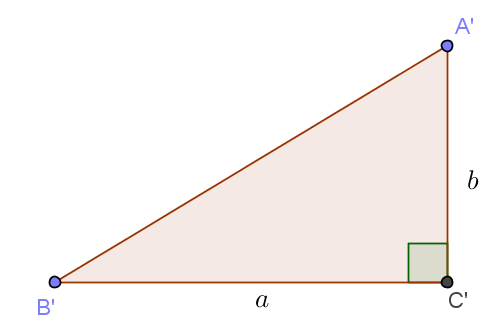
\includegraphics{3_5_2}
\caption{피타고라스 정리의 역에 대한 증명(2)}
\end{figure}
이 때, 삼각형 \(A'B'C'\)의 빗변의 길이를 \(x\)라고 하면 피타고라스의 정리로부터 \(a^2+b^2=x^2\)이 성립한다.
또 가정에서 \PP라고 했으므로 \(x^2=c^2\)이다.
그런데 \(x>0\), \(c>0\)이므로 \(x=c\)이다.
그러면 \(\triangle ABC\equiv\triangle A'B'C'\)(SSS 합동)이 된다.
따라서 \(\angle C=\angle C'=90\D\)이다.
\end{proof}

위의 증명 방식과는 다르게 간접적으로 증명할 수도 있다.
{\slshape증명}. (1) 처럼 직접적으로 증명하는 방법을 `직접증명법'이라고 말하고 앞으로 소개할 {\slshape증명}. (2)에서처럼 간접적으로 증명하는 방법을 `간접증명법'이라고 한다.
{\slshape증명}. (2)에서는 간접증명법 중에서도 `귀류법'이라는 증명방식을 사용했다.
\begin{proof}(2)
만약 \C=90\D가 아니라면 \C<90\D이거나 \C>90\D이어야 한다.
\C<90\D인 경우 \textbf{3.2}에 의해 \PPP가 되어 \PP라는 가정에 모순되므로 성립할 수 없다.
\C>90\D인 경우 \textbf{3.3}에 의해 \PPPP가 되어 \PP라는 가정에 모순되므로 성립할 수 없다.
따라서 \C=90\D일 수밖에 없다.
\end{proof}

%새 小節
\subsection{\PPP이면 \C<90\D이다.}
마찬가지로 귀류법을 이용해 증명할 수 있다.
\begin{proof}
만약 \C<90\D가 아니라면 \C=90\D이거나 \C>90\D이어야 한다.
\C=90\D인 경우 \textbf{3.1}에 의해 \PP가 되어 \PPP라는 가정에 모순되므로 성립할 수 없다.
\C>90\D인 경우 \textbf{3.3}에 의해 \PPPP가 되어 \PPP라는 가정에 모순되므로 성립할 수 없다.
따라서 \C<90\D일 수밖에 없다.
\end{proof}

%새 小節
\subsection{\PPPP이면 \C>90\D이다.}
\begin{proof}
만약 \C>90\D가 아니라면 \C=90\D이거나 \C<90\D이어야 한다.
\C=90\D인 경우 \textbf{3.1}에 의해 \PP가 되어 \PPPP라는 가정에 모순되므로 성립할 수 없다.
\C<90\D인 경우 \textbf{3.2}에 의해 \PPP가 되어 \PPPP라는 가정에 모순되므로 성립할 수 없다.
따라서 \C>90\D일 수밖에 없다.
\end{proof}

%새 節
\section{정리}
이상의 내용을 정리하면 다음과 같다.
삼각형\(ABC\)의 세 변을 각각 \(a\), \(b\), \(c\)라고 할 때,
\begin{gather*}
a+b>c\\
b+c>a\\
c+a>b
\end{gather*}
이 성립하고(삼각부등식), 또한
\begin{align*}
 \C=90\D&\iff\PP\\
 \C<90\D&\iff\PPP\\
 \C>90\D&\iff\PPPP.
\end{align*}
이 성립한다(피타고라스 정리 등).

%%새 節
%\section{참고한 책들}
%(1)
\end{document}